\documentclass[10pt,hyperref={CJKbookmarks=true},xcolor=dvipsnames,aspectratio=169]{beamer}
\usetheme[navigation]{UMONS}
\usepackage[utf8]{inputenc}
\usepackage{verbatim}
\usepackage{ctex}

\title[国际经济学]{国际经济学}
\subtitle{资本跨国流动:跨国公司理论}
\author{鲁晓东}
\institute[]{%
	岭南学院\hspace{2em}中山大学
	\\[4ex]
	
\includegraphics[height=8ex]{fig/lingnanlogo}\hspace{2em}%
	
\includegraphics[height=8.5ex]{fig/sysu}
}
%------------section前展示一页----------
\AtBeginSection[] {     
	\begin{frame}        
	\tableofcontents[currentsection,hideallsubsections]    
\end{frame} 
}

%-------------subsection也展示一下----------
\AtBeginSubsection[]{

\frame<beamer>{ 
	
	\frametitle{Outline}   
	
	\tableofcontents[currentsection,currentsubsection] 
	
}

}
%---------------------------

%-----------一段一闪现-------
%\beamerdefaultoverlayspecification{<+->}
%这个功能基本不用

\begin{document}
\maketitle


\begin{frame}
\frametitle{提纲}
\tableofcontents
\end{frame}				%生成提纲页

%-----------正文开始----------------------



\section{Motivation }
\begin{frame}{Motivation}

\begin{itemize}
\item international trade is not the only channel via which foreign demand
for cars is met 
\item Less than 50\% of Ford’s and Toyota’s production occurs in their countries
of origin
\begin{figure}


\begin{centering}
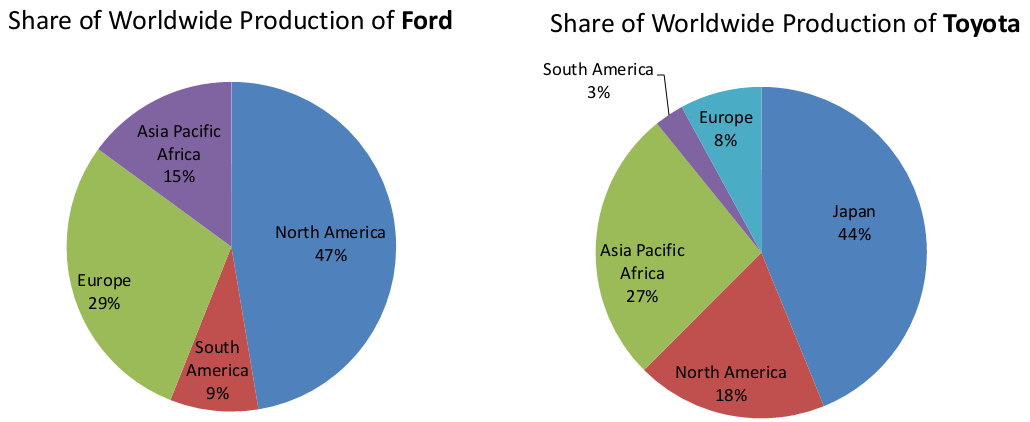
\includegraphics[width=10cm]{fig/fdi/lec7-1}
\par\end{centering}

\end{figure}

\end{itemize}
\end{frame}

\begin{frame}{Motivation }

\begin{itemize}
\item U.S. firms serve foreign markets mostly (75\%) via foreign affiliate
sales 
\begin{figure}


\begin{centering}
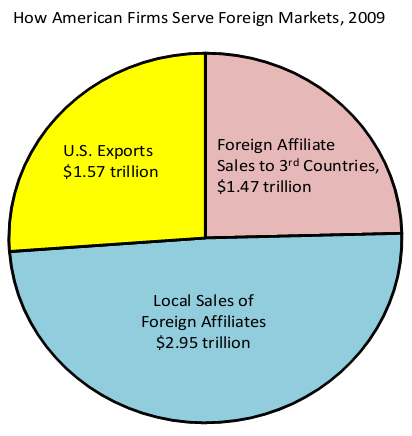
\includegraphics[width=5cm]{fig/fdi/lec7-2}
\par\end{centering}

\end{figure}

\end{itemize}
\end{frame}

\begin{frame}{Back to Boeing vs. Airbus }


\begin{figure}


\begin{centering}
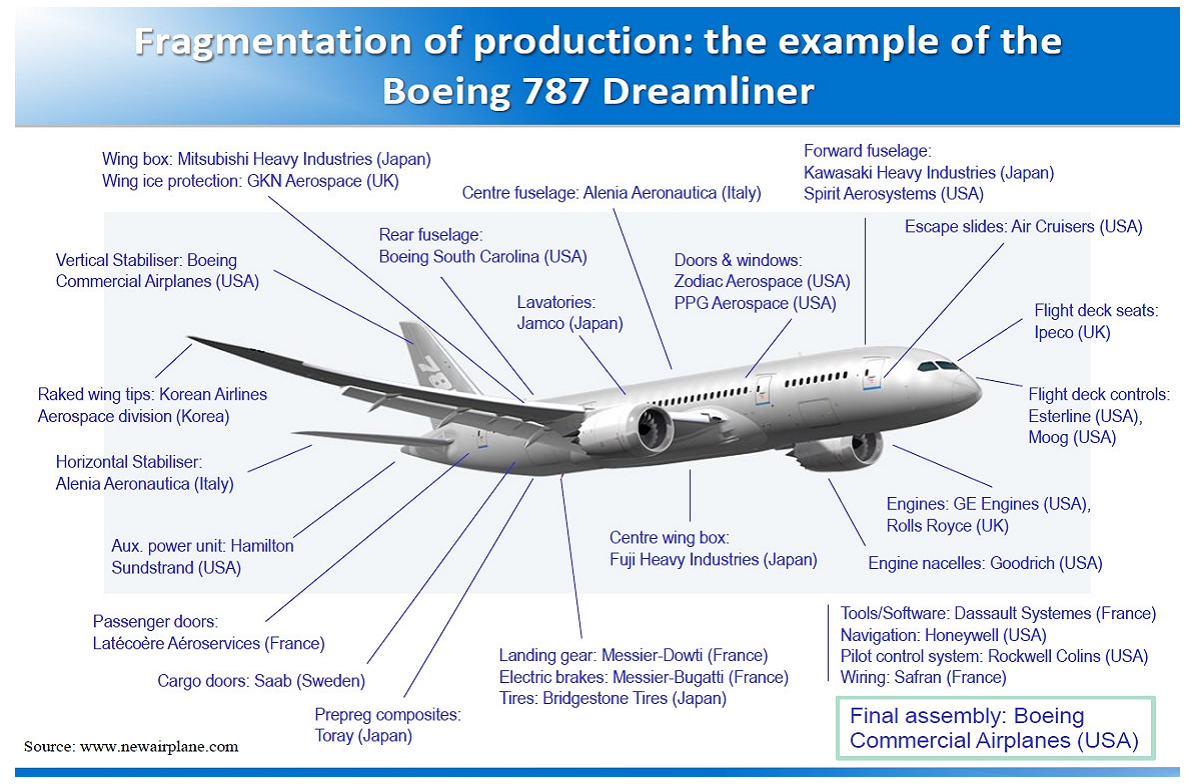
\includegraphics[width=10cm]{fig/fdi/glo12}
\par\end{centering}

\end{figure}

\begin{itemize}
\item 70 percent of the 787’s parts are produced in foreign countries 
\end{itemize}
\end{frame}

\begin{frame}{Importance of MNEs in U.S. Trade}

\begin{itemize}
\item Even when focusing on trade flows, understanding the behavior of MNEs
is important
\begin{figure}


\begin{centering}
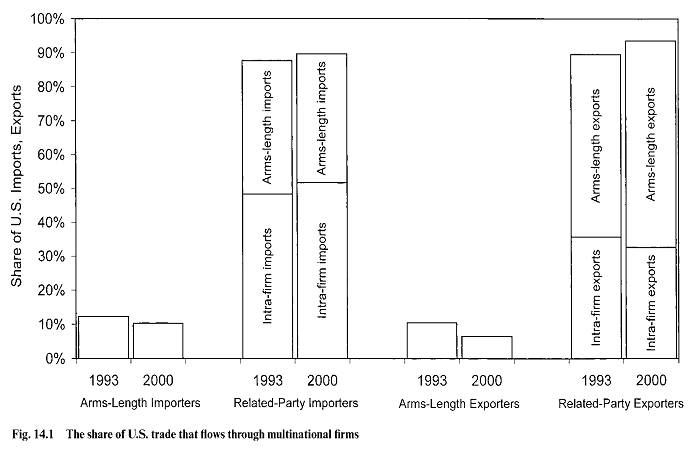
\includegraphics[width=8cm]{fig/fdi/lec7-3}
\par\end{centering}

\end{figure}

\end{itemize}

\end{frame}

\begin{frame}{Some Questions}

\begin{itemize}
\item Why do some firms “go global” and set up production abroad? 
\item Why do some firms opt out of that strategy? 
\item Why do some firms internalize (own/control) their production facilities
abroad while others do not? 
\item What is the effect of MNEs in their host countries? Do they exploit
labor?
\end{itemize}
\end{frame}

\section{Definitions, Broad Facts on MNEs}
\begin{frame}{Definitions }

\begin{itemize}
\item \textbf{\textcolor{cyan}{A multinational firm}} is “an enterprise
that controls and manages production establishments (plants) located
in at least two countries ” (Caves 1996, p. 1) 
\item Parent firm vs. affiliates or subsidiaries 
\item \textbf{\textcolor{cyan}{Foreign direct investment (FDI) }}flows are
made up of equity capital, reinvested earnings, and other capital
associated with an intercompany debt transaction (10\% equity stake
requirement) 
\item FDI flows might not be a good proxy for MNE activity 
\end{itemize}
\end{frame}

\begin{frame}{The Relevance of MNEs }


\begin{figure}


\begin{centering}
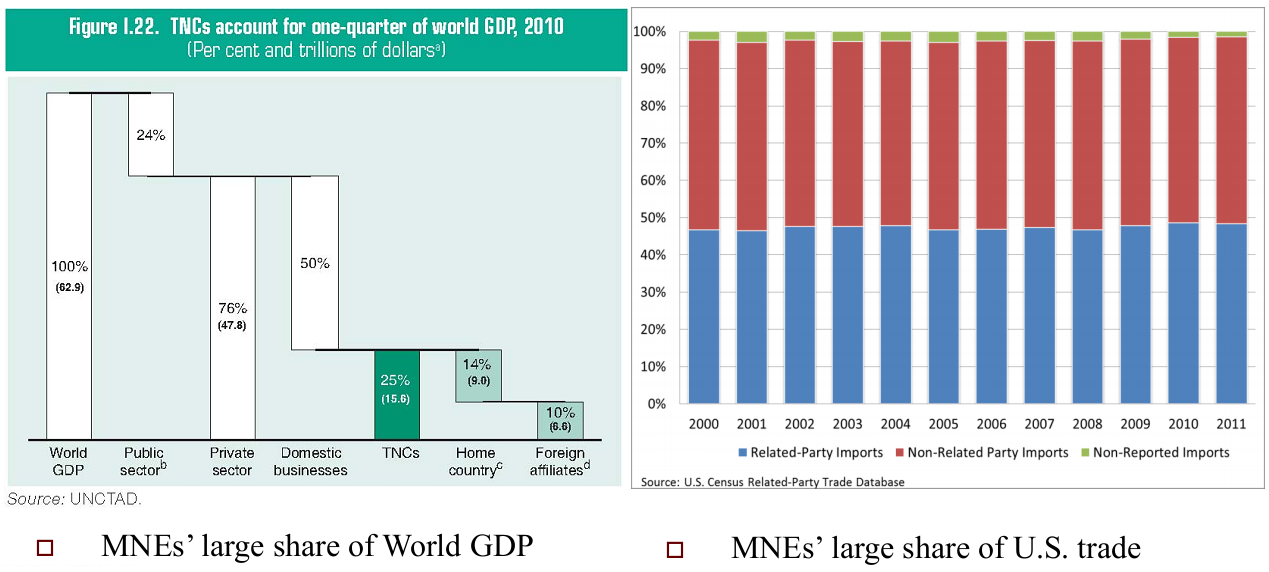
\includegraphics[width=12cm]{fig/fdi/glo13}
\par\end{centering}

\end{figure}



\end{frame}

\begin{frame}{Largest MNEs Are Very International }


\begin{figure}


\begin{centering}
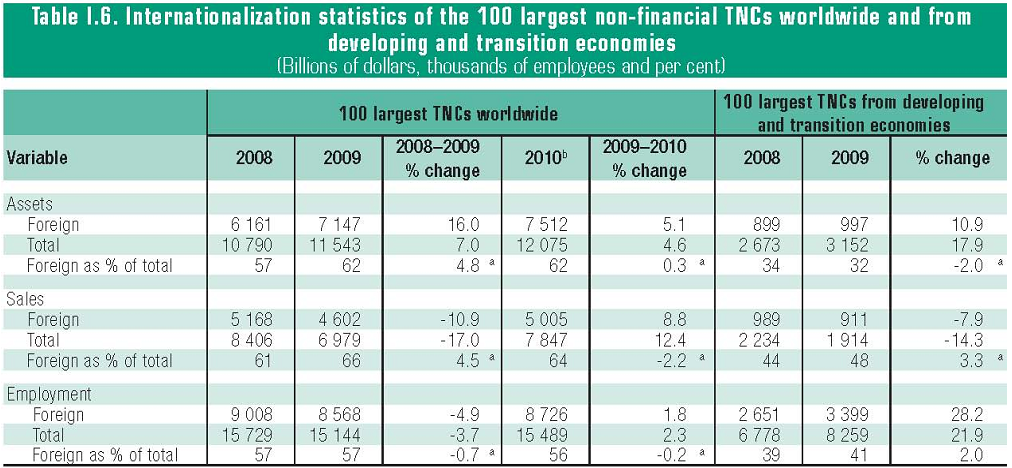
\includegraphics[width=11cm]{fig/fdi/lec7-4}
\par\end{centering}

\end{figure}

\end{frame}

\begin{frame}{Some Stylized Facts about MNEs }

\begin{itemize}
\item Some “Macro” Facts 

\begin{enumerate}
\item FDI and affiliate activity grew rapidly throughout the world, especially
in late 1980s, late 1990s and mid 2000s (but fell in recent crisis) 
\item Multinational activity is primarily concentrated in developed countries
where it is mostly two - way
\item Developing countries are more likely to be the destination of multinational
activity than the source
\item Political risk and instability deter inward FDI
\end{enumerate}
\end{itemize}
\end{frame}

\begin{frame}{Thirty Years of FDI Flows }


\begin{figure}


\begin{centering}
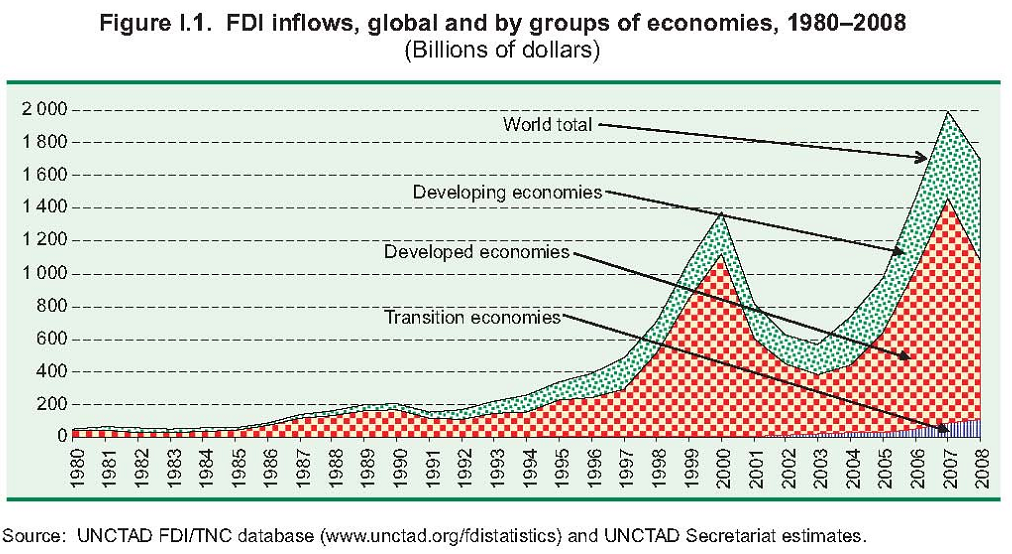
\includegraphics[width=12cm]{fig/fdi/lec7-5}
\par\end{centering}

\end{figure}



\end{frame}

\begin{frame}{Some Stylized Facts about MNEs }

\begin{itemize}
\item Firm and Industry Characteristics Common to MNEs 

\begin{enumerate}
\item High levels of R\&D expenditures over sales 
\item Employment of a large number of nonproduction (skilled) workers 
\item Production of new and/or complex goods 
\item High levels of product differentiation and advertising
\end{enumerate}
\end{itemize}
\end{frame}


\section{Why Go Global?}
\begin{frame}{Why Do Multinational Firms Exist? }

\begin{itemize}
\item Based on the starting definition this is due to the fact that a firm
decides to: 

\begin{itemize}
\item Locate part of the production process in a foreign country 地理位置
\item Take a “controlling” equity stake in the foreign production facility
所有权结构
\end{itemize}
\end{itemize}
\begin{enumerate}
\item \textbf{\textcolor{cyan}{Location}} : why is a good produced in at
least two countries rather than in just one country? 
\item \textbf{\textcolor{cyan}{Internalization}} : why is production in
different locations done by one firm rather that by separate firms? 
\item \textbf{\textcolor{cyan}{Non-Internalization}} : why is production in
different locations done by a third firms, say \textbf{\textcolor{cyan}{Offshoring Outsourcing}}?
\end{enumerate}
\end{frame}



\subsection{Location}
\begin{frame}{The Location Decision}

\begin{itemize}
\item Two main reasons for MNE activity to be profit-maximizing \end{itemize}
\begin{enumerate}
\item \textbf{\textcolor{cyan}{Horizontal FDI}}: When \textbf{\textcolor{blue}{exporting
is costly}}, replication of the production process in a foreign market
may be profit- maximizing (Nestlé, Toyota) 
\item \textbf{\textcolor{cyan}{Vertical FDI}}: In the presence of \textbf{\textcolor{blue}{factor
price (cost) differences}} across countries, a producer may find it
optimal to fragment production and undertake different parts/processes
in different countries 
\end{enumerate}
\end{frame}

\begin{frame}{Horizontal FDI: Model Setup}

\begin{itemize}
\item Consider the situation of a firm that is trying to decide how to best
service a foreign market 
\item One options:

\begin{itemize}
\item to increase production from the currently existing plant and export
this additional amount 
\item to set up an affiliate in the foreign market and avoid transportation
costs 
\end{itemize}
\item What is the cost of FDI? Suppose it entails additional \textbf{\textcolor{cyan}{fixed
costs}} associated with creating a new plant 
\item Exporting will also be costly, but most of the costs will be\textbf{\textcolor{cyan}{{}
variable }}in nature 
\end{itemize}
\end{frame}

\begin{frame}{Horizontal FDI: Predictions }

\begin{itemize}
\item Horizontal FDI will tend to dominate exporting in industries in which: 

\begin{itemize}
\item costs of transporting the goods internationally are high 
\item plant- level fixed costs are low relative to firm - level fixed costs
工厂层固定成本 V.S. 公司层固定成本
\item manmade tariff is hign enough
\end{itemize}
\item Furthermore, \textbf{\textcolor{blue}{a larger demand}} or \textbf{\textcolor{blue}{productivity
level}} (i.e., larger sales) will make horizontal FDI more attractive
relative to exporting 

\begin{itemize}
\item Easier to amortize the fixed cost of the new plant 
\item Firms facing low demand or featuring low productivity will opt out
of becoming multinationals 
\end{itemize}
\item Why positive effect of firm- level fixed costs? 
\end{itemize}
\end{frame}

\begin{frame}{Horizontal FDI: Evidence}


\begin{columns}[onlytextwidth]
\begin{column}{0.5\textwidth}
\begin{itemize}
\item Brainard (1997) found strong supportive evidence for the model (PSCALE工厂层规模经济,CSCALE公司层规模经济)
\item Helpman, Melitz and Yeaple (2004) confirmed the results and also showed
a negative effect of productivity on the ratio EXP/FDI 
\end{itemize}

\end{column}
\begin{column}{0.5\textwidth}
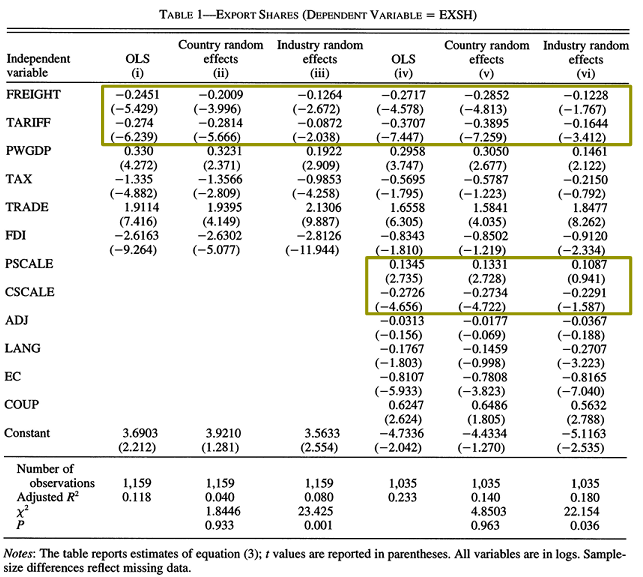
\includegraphics[width=\columnwidth]{fig/fdi/lec7-6}
\end{column}
\end{columns}

\end{frame}

\begin{frame}{Vertical FDI: Model Setup }

\begin{itemize}
\item Consider the situation of a firm that is trying to decide how to produce
a final good at minimum average cost 
\item The production process entails a skill - intensive process (R\&D,
product development…) and an unskilled - intensive process (assembly) 
\item One option is to concentrate both processes in the same plant or location 
\item An alternative is to set up an affiliate in a foreign market that
focuses on the production of a given process 
\end{itemize}
\end{frame}

\begin{frame}{Vertical FDI: Model Setup (cted.) }

\begin{itemize}
\item \textbf{\textcolor{blue}{What are the costs of FDI? }}

\begin{itemize}
\item Transportation costs involved in the cross - border exchange of inputs
\item coordination costs; communication costs
\item fixed costs 
\end{itemize}
\item \textbf{\textcolor{blue}{What are the benefits of FDI?}}

\begin{itemize}
\item Exploitation of cross- country differences in factor prices by shifting
production processes (with different input requirements) to locations
where they can be carried out more cheaply 
\end{itemize}
\item This is very much related to the concept of \textbf{\textcolor{blue}{comparative
advantage}} in Heckscher- Ohlin Model 
\end{itemize}
\end{frame}

\begin{frame}{Vertical FDI: Predictions }

\begin{itemize}
\item The model predicts that the prevalence of MNEs and FDI should be: 

\begin{itemize}
\item Decreasing in transportation costs (as well as coordination costs) 
\item Increasing in relative factor endowment differences across countries
(which generate factor price differences) 
\item Increasing in relative factor intensity differences across processes 
\end{itemize}
\item Notice also that while in Horizontal FDI models, trade and FDI are
\textbf{\textcolor{cyan}{substitutes … }}
\item ... here, Vertical FDI and trade are \textbf{\textcolor{cyan}{complements }}
\end{itemize}
\end{frame}

\begin{frame}{Vertical FDI: Evidence }


\begin{columns}[onlytextwidth]
\begin{column}{0.5\textwidth}
\begin{itemize}
\item Yeaple (2003) shows that U.S. MNEs favor skilled - abundant countries
over unskilled - abundant countries in skill intensive sectors 
\item But instead favor unskilled - abundant countries in unskilled - intensive
industries
\end{itemize}

\end{column}
\begin{column}{0.5\textwidth}
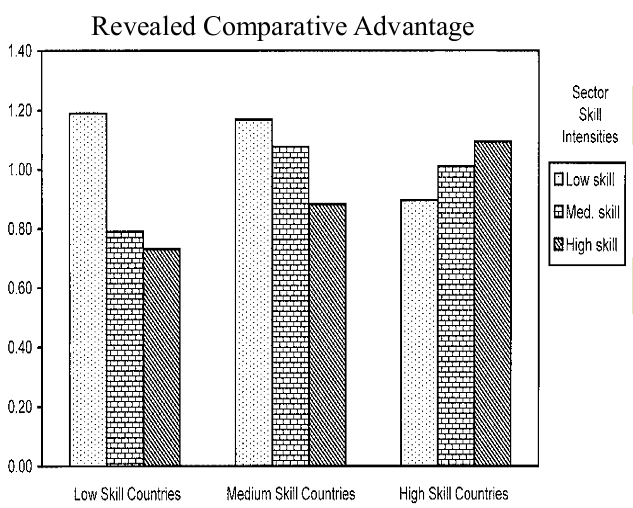
\includegraphics[width=\columnwidth]{fig/fdi/lec7-7}
\end{column}
\end{columns}

\end{frame}



\subsection{Internalization}
\begin{frame}{Internalization}

\begin{itemize}
\item In developing their global sourcing strategies, firms not only decide
on 

\begin{itemize}
\item \textbf{\textcolor{blue}{where }}to locate the different stages of
the value chain, 
\item but also on \textbf{\textcolor{blue}{the extent of control}} to exert
over them 
\item The issue of internalization or control is crucial for the existence
of MNEs 
\end{itemize}
\item But theories of location shed little light on the issue of internalization 

\begin{itemize}
\item why will fragmentation occur \textbf{\textcolor{blue}{within firm
boundaries}} ? 
\end{itemize}
\end{itemize}
\end{frame}

\begin{frame}{Theories of Internalization }

\begin{itemize}
\item \textbf{\textcolor{blue}{1. Costly technology transfer}}(转移理论): transfer
of knowledge or technology may be easier within a single organization
than through a market transaction (e.g., licensing) 

\begin{itemize}
\item Patent or property rights may be weak or non-existent
\item Knowledge may not be easily packaged and sold 

\begin{itemize}
\item Non -excludability 
\end{itemize}
\item Helps explain decision of Intel to own all its plants 
\end{itemize}
\end{itemize}
\end{frame}

\begin{frame}{Theories of Internalization }

\begin{itemize}
\item \textbf{\textcolor{blue}{2. Vertical integration}}(契约理论): consolidation
of different stages of a production process 

\begin{itemize}
\item Intrafirm purchases may avoid or attenuate contractual difficulties
契约失灵
\item Integration may affect the relative bargaining power and incentives
of producers and suppliers in a profit - enhancing way
\end{itemize}
\item May explain why Toyota internalizes certain upstream production stages,
while Nike doesn’t
\end{itemize}
\end{frame}

\begin{frame}{Empirical Evidence }

\begin{itemize}
\item Tests of the internalization decision are harder to come by due to
data limitations 
\item Some authors have used data on\textbf{\textcolor{blue}{{} licensing
arrangements}} to test the costly transfer theory 许可证手段
\item Others have used\textbf{\textcolor{blue}{{} intrafirm trade data}} to
test contractual theories of vertical integration 企业内部贸易数据
\item The latter is easily accessible (at least for the U.S.) and offers
a broad picture of internalization patterns

\begin{itemize}
\item As exemplified by the following few graphs
\end{itemize}
\end{itemize}
\end{frame}

\begin{frame}{Variation in Intrafirm Trade }


\begin{figure}


\begin{centering}
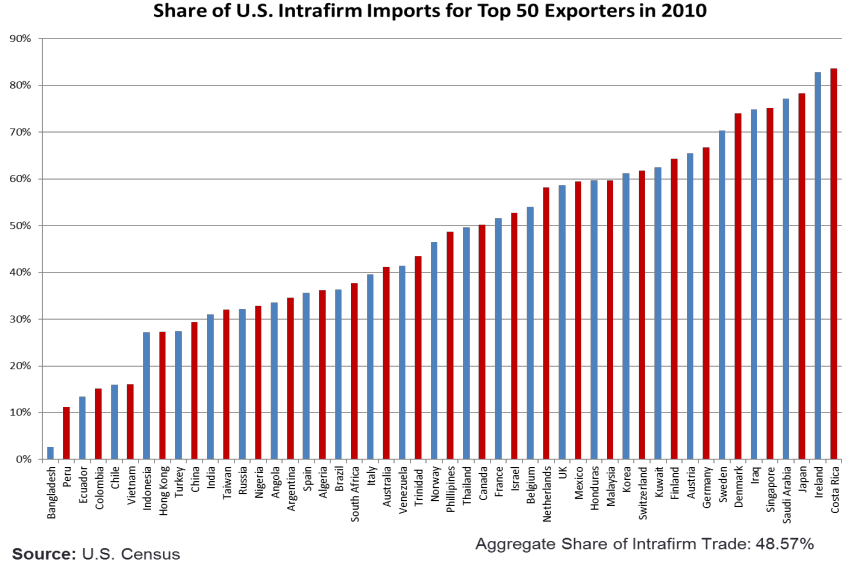
\includegraphics[width=10cm]{fig/fdi/lec7-8}
\par\end{centering}

\end{figure}

\end{frame}

\begin{frame}{Variation in Intrafirm Trade}


\begin{figure}


\begin{centering}
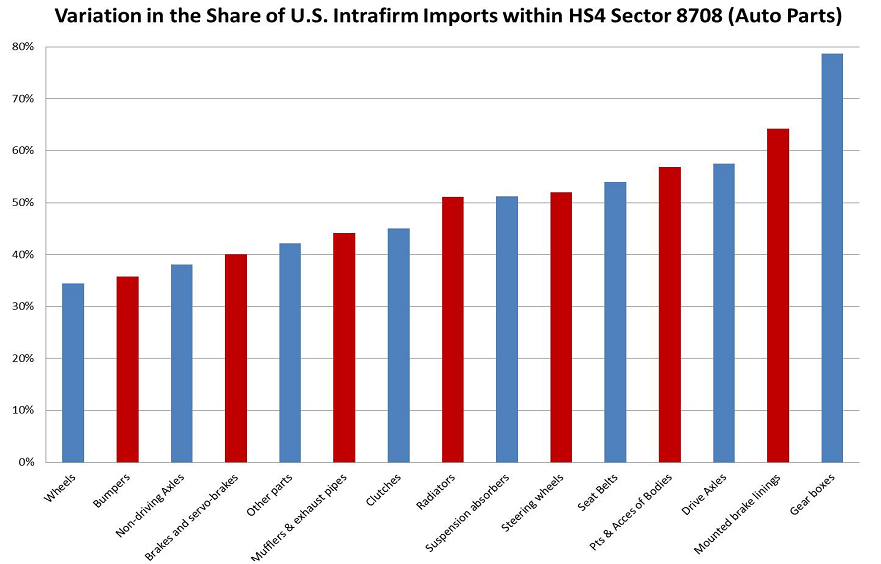
\includegraphics[width=10cm]{fig/fdi/lec7-9}
\par\end{centering}

\end{figure}

\end{frame}

\begin{frame}{Variation in Intrafirm Trade}


\begin{figure}


\begin{centering}
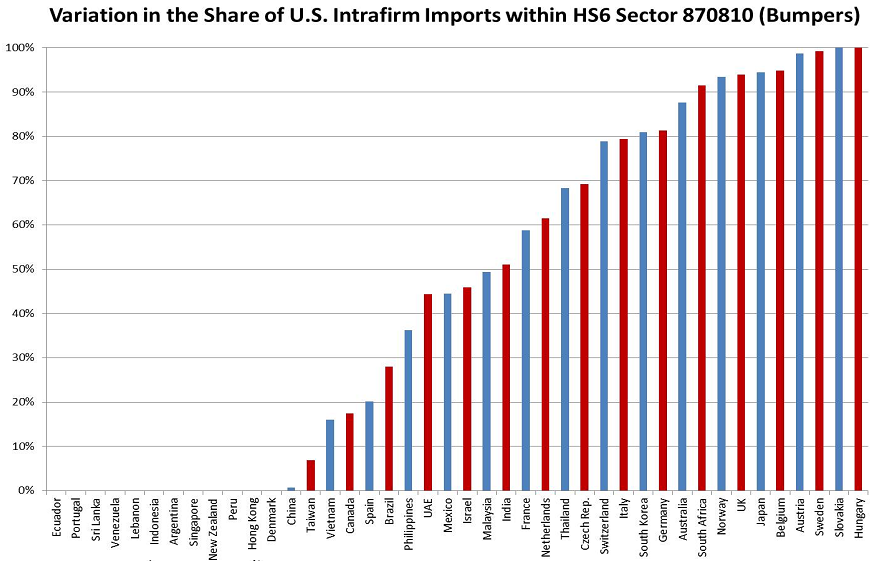
\includegraphics[width=9cm]{fig/fdi/lec7-10}
\par\end{centering}

\end{figure}

\end{frame}

\begin{frame}{Internalization: Some Evidence }


\begin{figure}


\begin{centering}
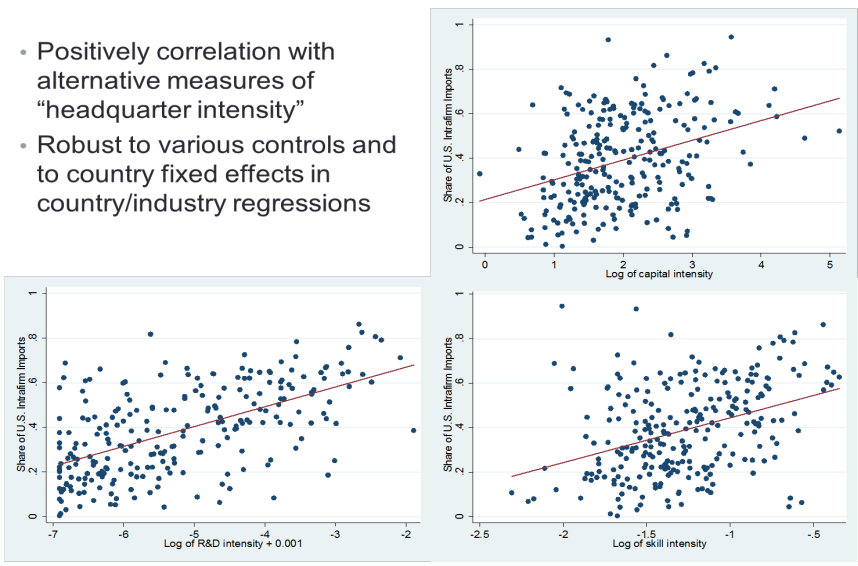
\includegraphics[width=10cm]{fig/fdi/lec7-11}
\par\end{centering}

\end{figure}

\end{frame}

\subsection{offshoring outsourcing}

\begin{frame}{何为外包}

 \begin{block}{}
	不断增长的服务贸易一方面是离岸外包业务量的上升。通过外包,企业能够将劳动密集型服务产业的功能转移到其他国家……当一种产品或服务在国外生产成本更低时,进口该种产品或服务比在国内生产更为明智和有利。\\
	--2004年《总统经济报告》,第229页
	
\end{block}
  \begin{itemize}
  	\item 对垂直型FDI的一种替代,是Internalization策略的一种反向操作
  	\item 问题:对于水平型FDI的替代形式是什么?
    \item 境外外包(foreign outsourcing):一项服务由一个国家提供并由另一个国家使用,或者一件商品的各个部件在不同国家生产然后在另一国家完成装配的现象,又称为外包(outsourcing)
    
  \end{itemize}

\end{frame}

\begin{frame}{外包和垂直专业化之间的权衡}
 \begin{block}{}
 	许多理论可以归结为不同的成本节约和转移部分生产程序到海外的固定成本之间的权衡
 \end{block}
  \begin{itemize}
  	\item 决定内部化的关键因素——所有者优势
  	\item 外包的主要收益———节约成本,并获取规模优势
  \end{itemize}
\end{frame}

\begin{frame}{参与离岸外包的公司是否是出口公司}
	\begin{itemize}
		\item 或者说进口商同时也是出口商吗?
		\item 美国92\%的公司(以就业来衡量)既进口中间品又进行出口
		\item 中国的情况
	\end{itemize}
	\begin{table}
		\centering
		\caption{进口企业同时也是出口企业}
		\begin{tabular}{llll} 
			\hline
			出口类型   & 数量(个)  & 比例(\%) & 累积比例   \\ 
			\hline
			既出口又进口 & 27,686 & 64.25  & 64.25  \\
			仅仅出口   & 14,375 & 33.36  & 97.6   \\
			仅仅进口   & 1,033  & 2.4    & 100    \\
			\hline
		\end{tabular}
	\end{table}
\end{frame}

\section{The Economic Impact of MNEs }
\begin{frame}{Effects on the Labor Market}

\begin{itemize}
\item Brown, Deardorff and Stern (2003): “the popular press is rife with
anecdotes about foreign workers who labor for multinational firms
for low wages and for excruciating long hours under horrific conditions
in low - income countries” (p. 51). 跨国公司被诟病最多的是:低工资和血汗工厂
\item It is common to refer to the practices of MNEs and their subcontractors
as “unfair” (especially given the high ratio of retail prices to labor
costs)零售价格和劳动成本严重不成比例 
\item Is the solution to restrict MNE activity or out-sourcing? 
\end{itemize}
\end{frame}

\begin{frame}{What is the Counterfactual?}

\begin{itemize}
\item \textbf{\textcolor{blue}{Key Question}} : what would happen if workers
in LDCs could only be employed by domestic firms? 
\item Evidence suggests that workers employed in MNEs in LDCs are paid wages
that are on average higher than those paid by domestic firms 
\item Particular studies include Glewwe (2000) for Vietnam, Aitken et al.
(1996) for Mexico, Lipsey and Sjoholm for Indonesia
\end{itemize}
\end{frame}

\begin{frame}{Rough Evidence from Vietnam }

\begin{itemize}
\item Average wages appear to be significantly higher in foreign - owned
businesses (FOB) 
\begin{figure}


\centering{}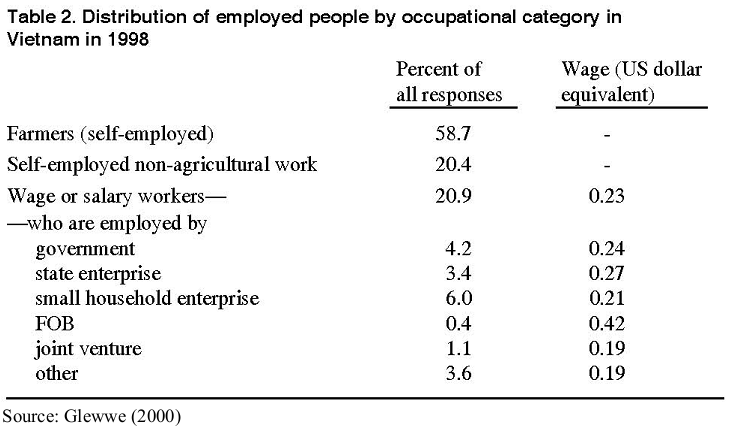
\includegraphics[width=10cm]{fig/fdi/lec7-12}
\end{figure}

\item Is this measurement can justify the MNEs?这个测算有什么问题?
\end{itemize}
\end{frame}

\begin{frame}{Not So Straightforward A Comparison}

\begin{itemize}
\item Type of workers that MNEs hire may be different from type of workers
that domestic firms hire 

\begin{itemize}
\item MNEs hire higher skilled workers 
\end{itemize}
\item This is problematic because the relevant “alternative wage” for MNE-
employed workers might be higher than that of the average domestic
worker 
\item How does one deal with this selection problem? 
\item \textbf{\textcolor{blue}{Ideal experiment}}: take two twin brothers
and randomly assign them to two comparable firms except for their
countries of ownership 
\item In practice, control for firm or individual fixed effects 
\end{itemize}
\end{frame}

\begin{frame}{Refinement \#1}

\begin{itemize}
\item Control for average worker characteristics and firm characteristics 
\item Foreign-Owned wage premium remains but appears smaller
\begin{figure}


\begin{centering}
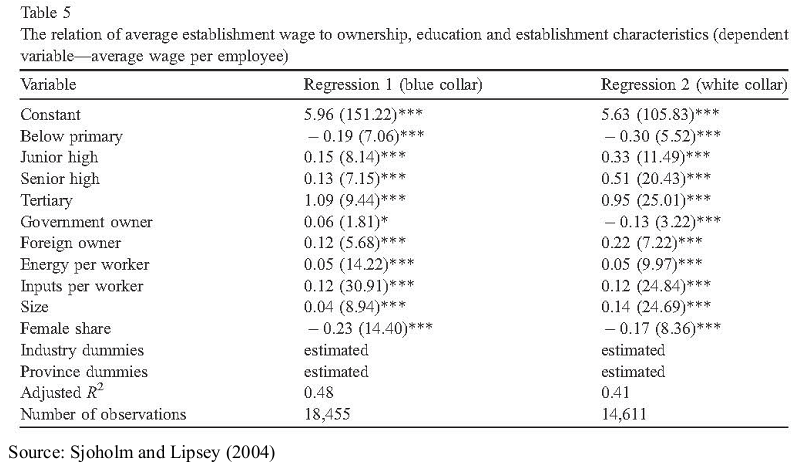
\includegraphics[width=10cm]{fig/fdi/lec7-13}
\par\end{centering}

\end{figure}

\end{itemize}
\end{frame}

\begin{frame}{Refinement \#2}

\begin{itemize}
\item Use within-establishment comparison (i.e., takeovers). Again premium
survives 
\begin{figure}


\begin{centering}
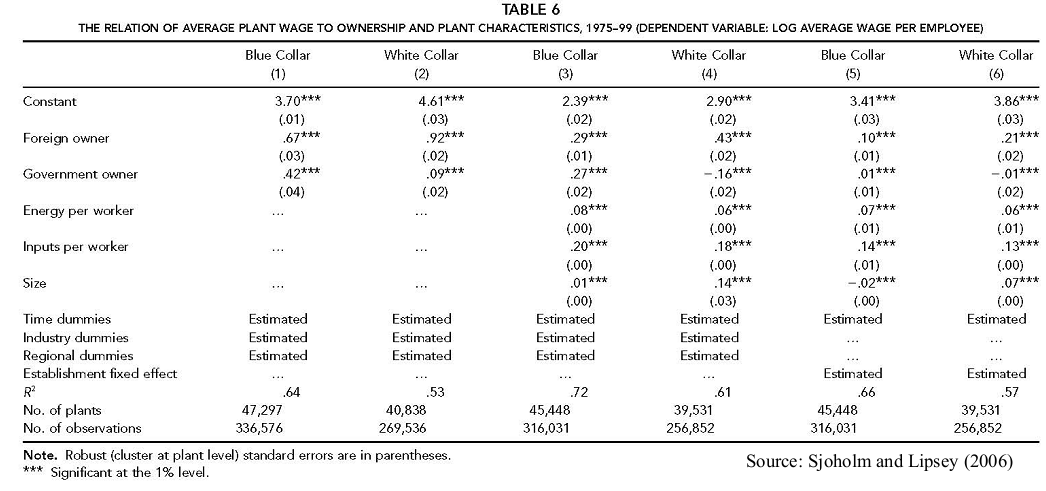
\includegraphics[width=11cm]{fig/fdi/lec7-14}
\par\end{centering}

\end{figure}

\end{itemize}
\end{frame}

\begin{frame}{Refinement \#3 }

\begin{itemize}
\item Use individual worker data rather than firm averages (Swedish data)
\begin{figure}


\begin{centering}
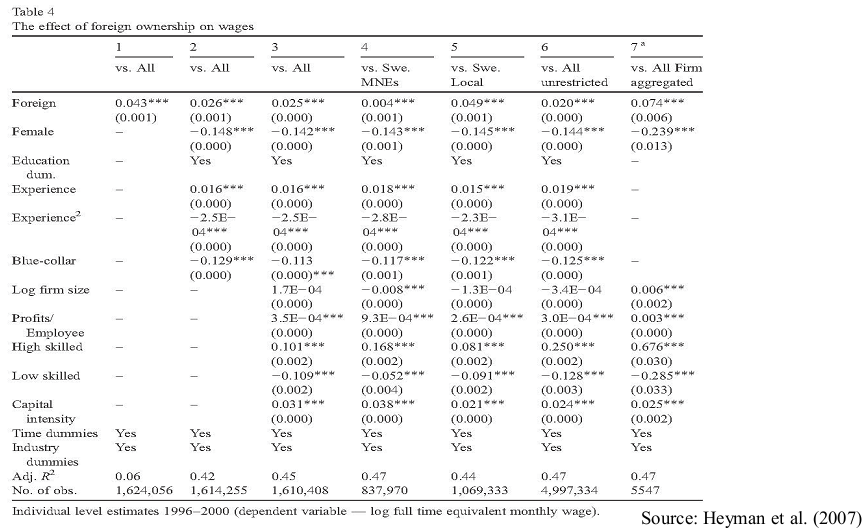
\includegraphics[width=10cm]{fig/fdi/lec7-15}
\par\end{centering}

\end{figure}

\end{itemize}
\end{frame}

\begin{frame}{Refinement \#4 }

\begin{itemize}
\item Again look at the effects of takeovers. Premium close to gone! But
was the takeover random? 
\begin{figure}


\centering{}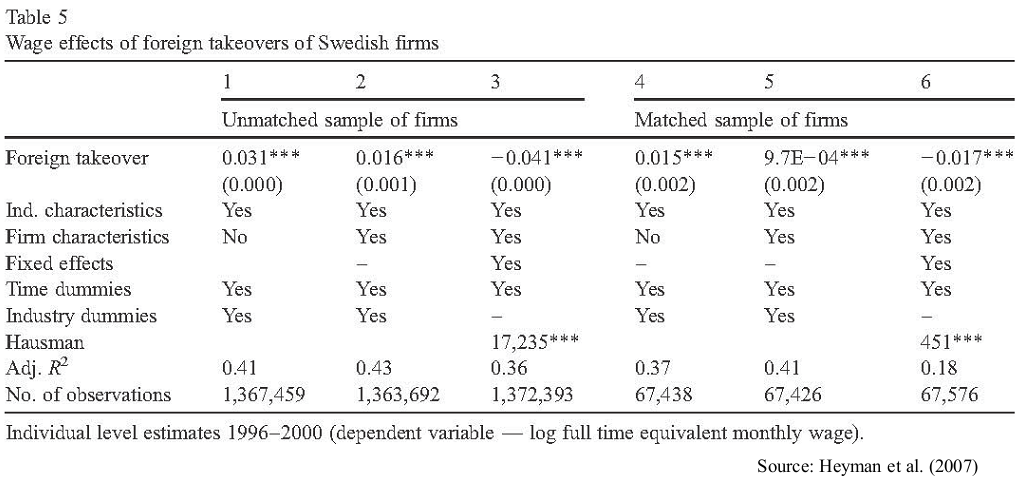
\includegraphics[width=11cm]{fig/fdi/lec7-16}
\end{figure}

\end{itemize}
\end{frame}

\begin{frame}{Effects on Wage Levels }

\begin{itemize}
\item A more fundamental question is what is the effect of MNEs on \textbf{\textcolor{blue}{average}}
host - country wages 东道国的平均工资水平

\begin{itemize}
\item MNEs could lead to a large increase in average wages, with a disproportionate
positive effect on workers employed in domestic firms 
\end{itemize}
\item Theoretically, the effect is unclear: 

\begin{itemize}
\item If MNE implies capital or technology inflow, or increased trade integration
(fragmentation), then one would expect positive effect on wages (rule
out factor price insensitivity)
\item If MNEs are monopsonists in labor markets, then there could be perverse
effects 
\end{itemize}
\end{itemize}
\end{frame}

\begin{frame}{Effects on Wage Levels: Evidence}

\begin{itemize}
\item Aitken et al. (1996) find that MNEs have a positive impact on host
- country wages… 
\item …but that this positive effect tends to be concentrated among the
set of workers that are employed by these MNEs 
\item Their results indicate that skilled workers tend to benefit more than
unskilled workers from FDI 

\begin{itemize}
\item result confirmed by a variety of studies 
\item problematic for standard models of vertical fragmentation
\end{itemize}
\end{itemize}
\end{frame}

\begin{frame}{Effects on Capital Markets}

\begin{itemize}
\item Not too much work on this issue 
\item Feldstein (1995): “How much does the U.S. domestic capital stock decline
per dollar of additional capital in foreign affiliates of U.S. multinationals?” 
\item Key issues: Do portfolio investment inflows compensate for part of
these outflows? How much financing of affiliates comes from U.S.? 
\item Answers are: “No” and “Little”. Overall only about 20 - 40 cents are
“lost” 
\item Desai, Foley and Hines (2005) find a complementarity at the firm level
(more investment abroad → more investment at Home) 
\end{itemize}
\end{frame}

\begin{frame}{Spillover Effects}

\begin{itemize}
\item There are several reasons for why FDI should affect productivity of
local firms in host countries

\begin{enumerate}
\item Domestic firms may benefit from increased technological diffusion
if foreign affiliates located in that country\textbf{\textcolor{blue}{{}
introduce new products or processes 新产品新工艺}}
\item Productivity may increase simply from host-country firms \textbf{\textcolor{blue}{observing}}
how production takes place in local affiliates of foreign firms 学习
\item FDI may toughen the competition faced by domestic firms, thereby forcing
them to “\textbf{\textcolor{blue}{trim their fat}}” and become more
competitive 竞争
\item 4. Productivity spillovers via \textbf{\textcolor{blue}{labor turnover
		劳动力培训}}

\begin{itemize}
	\item former employees of multinational firms set up their own businesses
	and adopt some of the techniques they were using in the foreign firm 
\end{itemize}
\item 5. FDI can generate positive spillovers by increasing local demand
for intermediate inputs, hence allowing suppliers to \textbf{\textcolor{blue}{move
		down along their average curve}} 后向关联
\item 6. By the same argument, FDI can decrease the productivity of domestic
firms operating in the same sector because the “business -stealing”
effect may \textbf{\textcolor{blue}{increase average costs 副作用,本土企业产出减少,成本上升}}
\end{enumerate}
\end{itemize}
\end{frame}



\begin{frame}{Spillover Effects: Evidence }

\begin{itemize}
\item Aitken and Harrison (1999) estimate the productivity effects of inward
FDI on a sample of Venezuelan manufacturing plants in the period 1976-
1989 
\item Although the average effect of FDI on plant productivity is positive,
domestic firms in sectors with larger foreign presence actually record
lower productivity levels 

\begin{itemize}
\item So average effect is purely coming from foreign firms being more productive
整体生产率上升的真正原因是FDI的流入,而非由于溢出效应带来本土企业生产率上升
\end{itemize}
\end{itemize}
\end{frame}

\begin{frame}{Spillover Effects: Evidence (cted.) }

\begin{itemize}
\item Other authors have found positive horizontal spillover effects in
other countries (i.e., UK) 
\item Smarzynska (2004) argues that spillovers from FDI are more likely
to be vertical than horizontal in nature 垂直FDI更可能发生溢出

\begin{itemize}
\item she finds that the positive effects of FDI take place mostly through
backward linkages, with a negligible effect of FDI through either
horizontal or forward linkages 
\item So local suppliers become more productive when MNEs enter a country 
\end{itemize}
\end{itemize}
\end{frame}

\begin{frame}{Next Time}

\begin{itemize}
\item Begin the analysis of the causes and consequences of trade policy 
\item have fun!
\end{itemize}
\end{frame}

\end{document}
